% !TeX root = thesis.tex

\chapter{Background} \label{chap:background}

This chapter introduces the technological background required to understand the industrial process addressed in this dissertation. It first presents the 
fundamentals of biogas production and upgrading technologies, followed by a description of the VPSA process employed in the 
considered biomethane plant. Finally, the vacuum pump, which constitutes the main asset analysed in this work, is presented together with its operating principle, 
instrumentation, maintenance procedures, and common faults.

\section{What is Biogas?} \label{sec:biogasupgrading}

Biogas is a renewable gaseous fuel produced through the anaerobic digestion of biodegradable 
organic matter, a biological process in which microorganisms decompose organic 
compounds in the absence of oxygen. This process converts complex organic materials 
into simpler compounds while producing a gaseous mixture known as biogas. A wide 
range of feedstocks can be used for anaerobic digestion, including agricultural 
residues, livestock manure, municipal solid waste, sewage sludge, food waste, and 
other types of organic biomass, as illustrated in Figure~\ref{fig:biogas_sources}.

\begin{figure}[htbp]
    \centering
    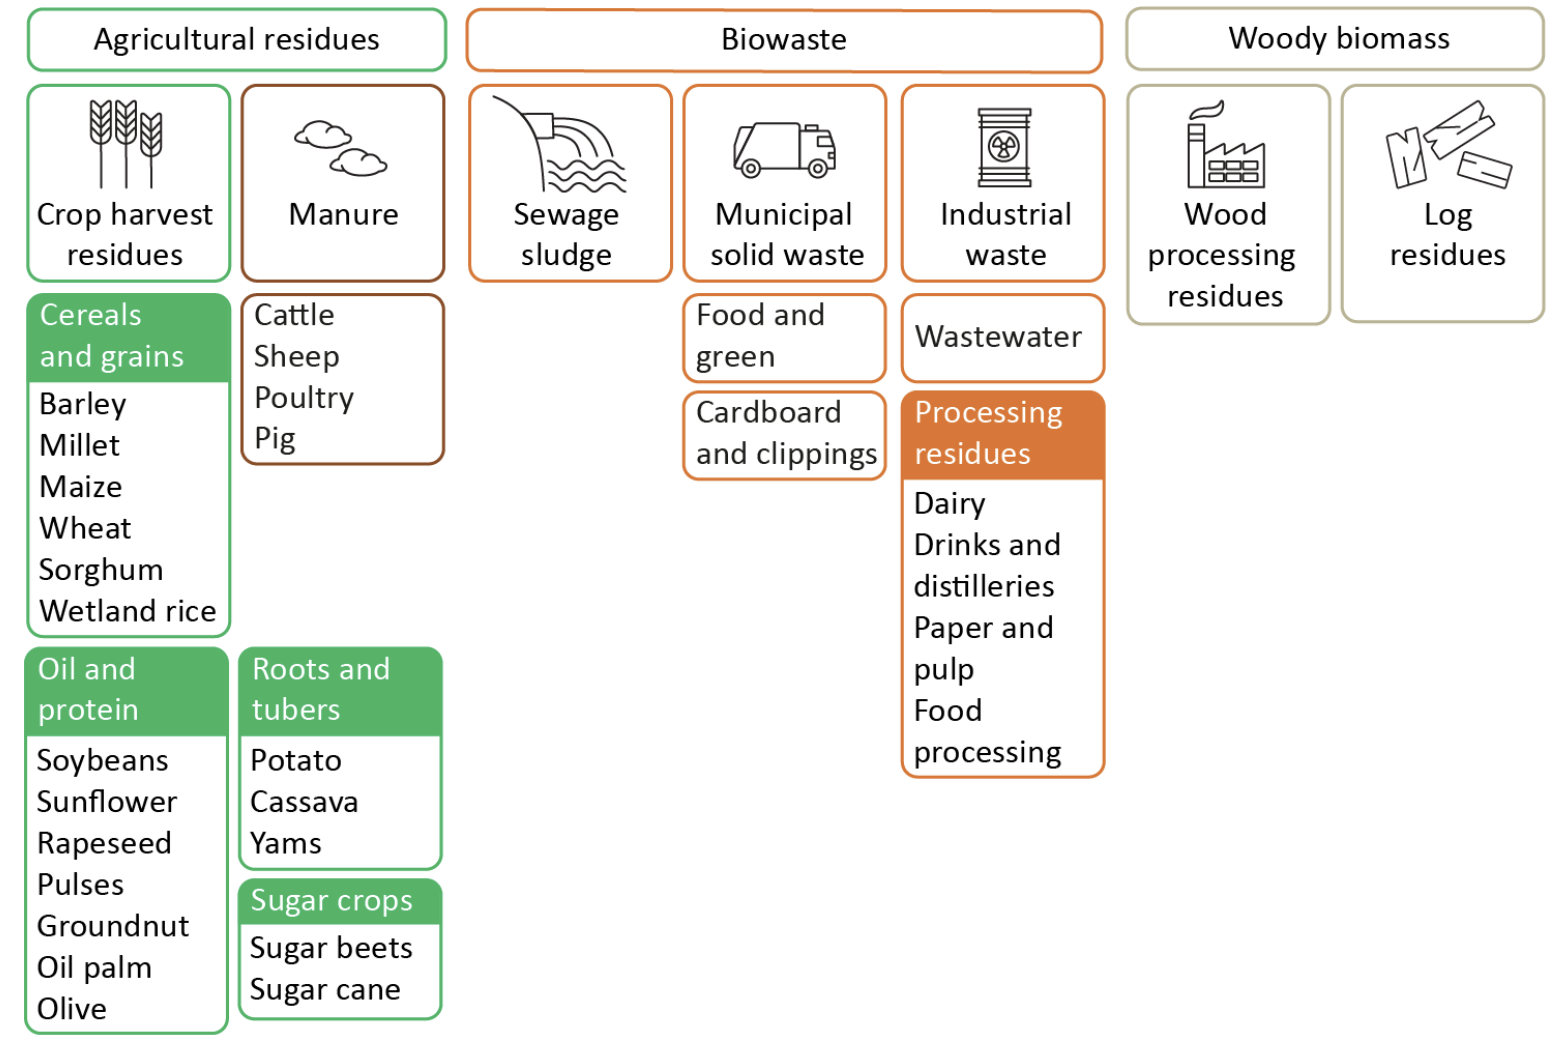
\includegraphics[width=0.8\textwidth]{imgs/biogas sources v2.png}
    \caption{Sources of organic waste feedstock for biogas production. Source: \cite{InternationalEnergyAgency2020}}
    \label{fig:biogas_sources}
\end{figure}

The composition of biogas depends on the type of feedstock and the 
operating conditions of the anaerobic digestion process. It is 
primarily composed of methane (CH$_4$), typically accounting for 
50--80\% of its volume, and carbon dioxide (CO$_2$), which 
represents approximately 20--50\%. In addition to these major 
constituents, biogas contains smaller concentrations of 
impurities, including hydrogen sulfide (H$_2$S), water 
vapour (H$_2$O), ammonia (NH$_3$), oxygen (O$_2$), and siloxanes.


Since methane is the component responsible for the calorific value, 
the relatively high concentration of carbon dioxide and 
other contaminants limits the direct use of raw biogas in many 
applications. Consequently, purification processes are required 
to increase its methane content and produce biomethane with 
properties comparable to those of natural gas (\cite{Swinbourn2024}). 


\section{Biogas Upgrading} \label{sec:biogasupgrading}

Biogas upgrading, also referred to as biogas purification, biogas refinement or biogas methanation, is the process of increasing the methane 
concentration of raw biogas by removing carbon dioxide and other undesirable contaminants. The resulting methane-rich gas, 
known as biomethane, has a significantly higher calorific value and can be used as a substitute for natural gas in a wide 
range of applications. In general, biomethane should contain at least 95\% methane to comply with the quality requirements 
for grid injection and other energy applications (\cite{Swinbourn2024}).

\begin{figure}[htbp]
    \centering 
    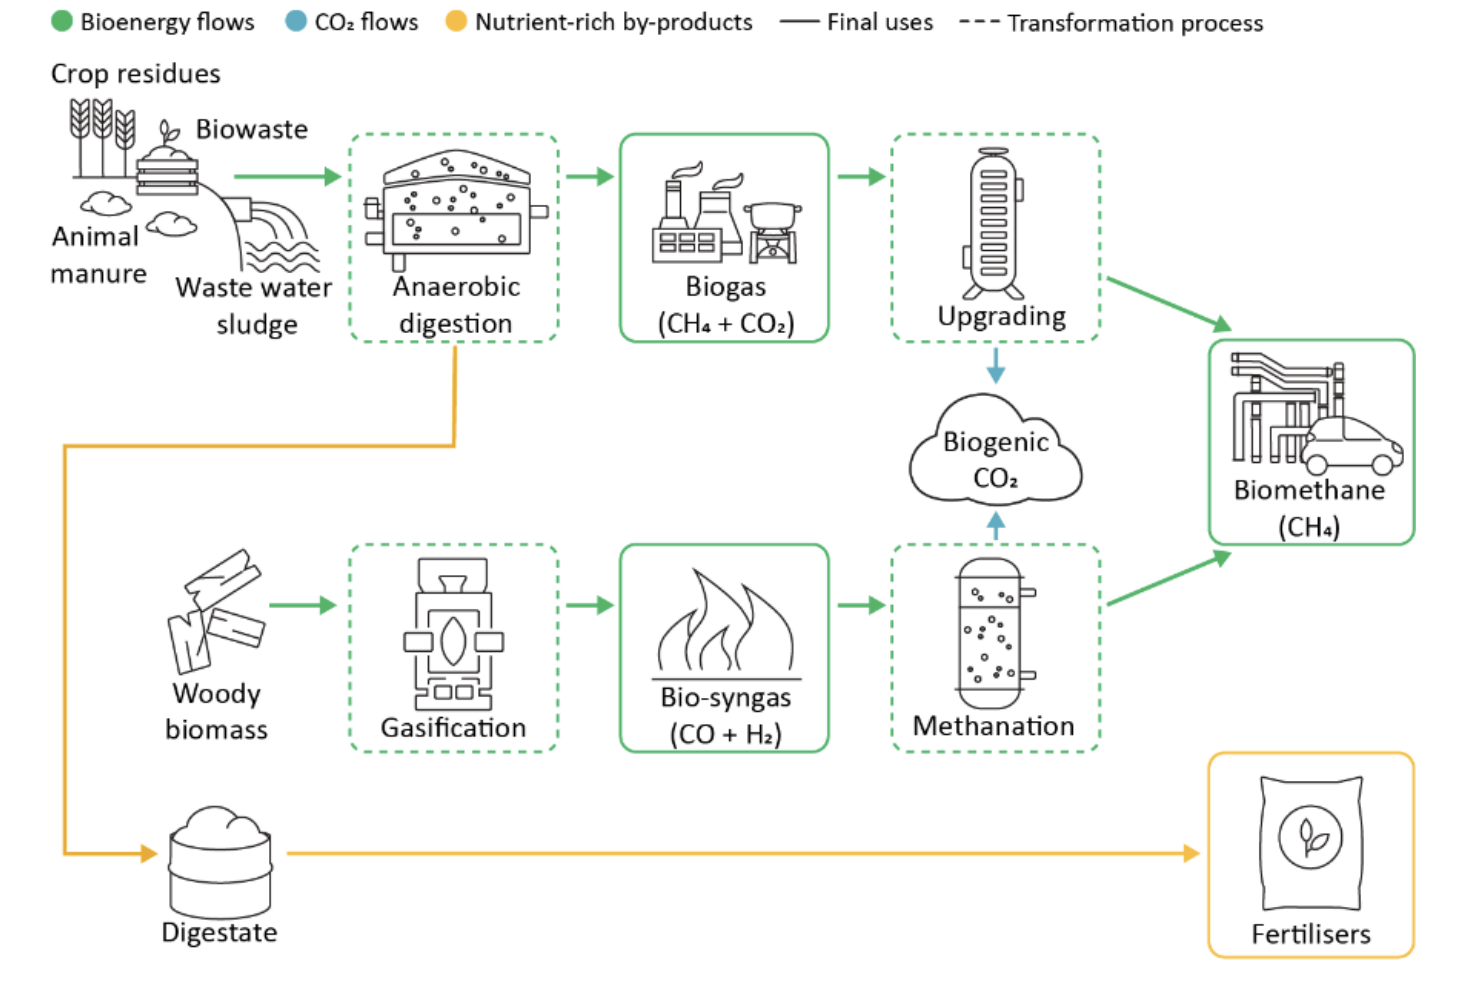
\includegraphics[width=0.8\textwidth]{imgs/upgrading.png}
    \caption{Biogas upgrading and utilization. Source: \cite{InternationalEnergyAgency2020}}
    \label{fig:biogas_sources}
\end{figure}

Several upgrading technologies have been developed to achieve this objective, each presenting different advantages, 
limitations, and operating requirements. Since a detailed comparison of these technologies is beyond the scope of this dissertation, 
only a brief overview of the main biogas upgrading methods is provided in the following section.

\subsection{Biogas Upgrading Technologies} \label{sec:biogastech}

The most widely adopted methods can be broadly classified into adsorption, membrane separation, cryogenic separation, and absorption processes (\cite{Naquash2025}):

\begin{itemize}
    \item \textbf{Adsorption separation:} One of the most widely used methods for biogas upgrading. Adsorption processes can be further classified into Pressure Swing Adsorption (PSA), Temperature Swing Adsorption (TSA), and Electric Swing Adsorption (ESA), with PSA being the most widely adopted. In PSA systems, biogas is compressed and passed through one or more columns filled with an adsorbent material. The adsorbent selectively retains contaminants while methane passes through the column. Once saturated, the column is regenerated by depressurization, allowing the adsorbed gases to be released before starting a new adsorption cycle.

    \item \textbf{Membrane separation:} This method uses semi-permeable membranes, typically made of polymeric materials, to separate methane from carbon dioxide and other impurities according to their different permeation rates. The membrane material and configuration depend on the desired biomethane purity.

    \item \textbf{Cryogenic separation:} Cryogenic upgrading exploits the different boiling points of the gas components. By progressively reducing the temperature, carbon dioxide and other contaminants condense before methane, allowing their separation.

    \item \textbf{Absorption separation:} Absorption processes use a liquid solvent, such as water or chemical solvents, to selectively absorb carbon dioxide from biogas. Water scrubbing is one of the most common upgrading technologies, taking advantage of the significantly higher solubility of carbon dioxide compared to methane under standard operating conditions.
\end{itemize}

Figure~\ref{fig:upgrading_technologies} summarizes the four main biogas upgrading technologies discussed in this section.

\begin{figure}[htbp]
    \centering
    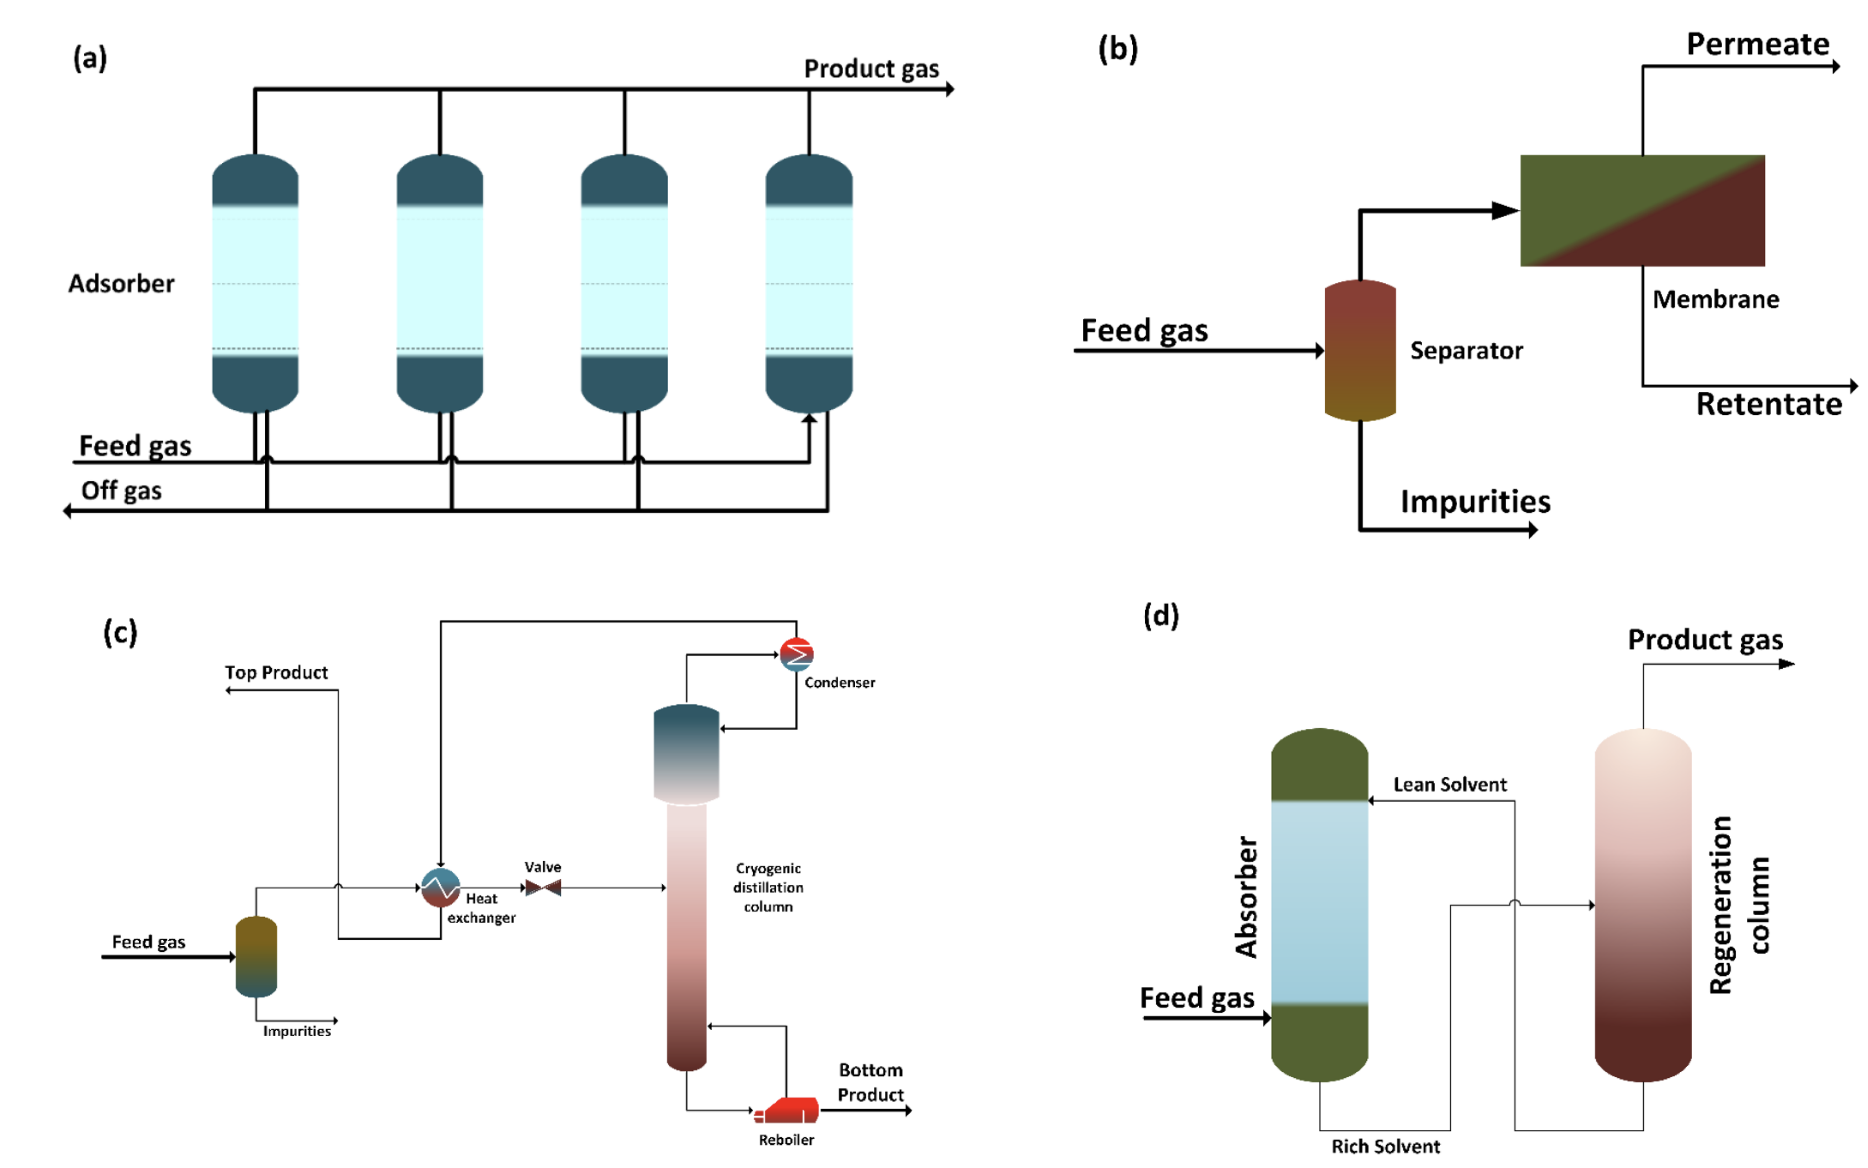
\includegraphics[width=0.85\textwidth]{imgs/upgrading technologies.png}
    \caption{Main biogas upgrading technologies: adsorption, membrane separation, cryogenic separation, and absorption. Source: \cite{Naquash2025}.}
    \label{fig:upgrading_technologies}
\end{figure}

Among the available technologies, a PSA biomethane upgrading plant was considered in this dissertation. Since the proposed AI models are developed 
using data collected from a PSA-based upgrading system, the following section presents a more detailed description of its operating principles and process 
configuration.

\section{Considered Biomethane Plant} \label{sec:biomethaneplant}

As discussed in the previous section, the biomethane upgrading plant considered in this dissertation employs PSA technology. More specifically, the plant operates using a four-column adsorption cycle and incorporates a 
vacuum pump during the regeneration stage to enhance the desorption of the adsorbed gases. This configuration is commonly 
referred to as Vacuum Pressure Swing Adsorption (VPSA).

A photograph of an example biomethane upgrading plant used in this work is presented in Figure~\ref{fig:metagenad}. 

\begin{figure}[htbp]
    \centering
    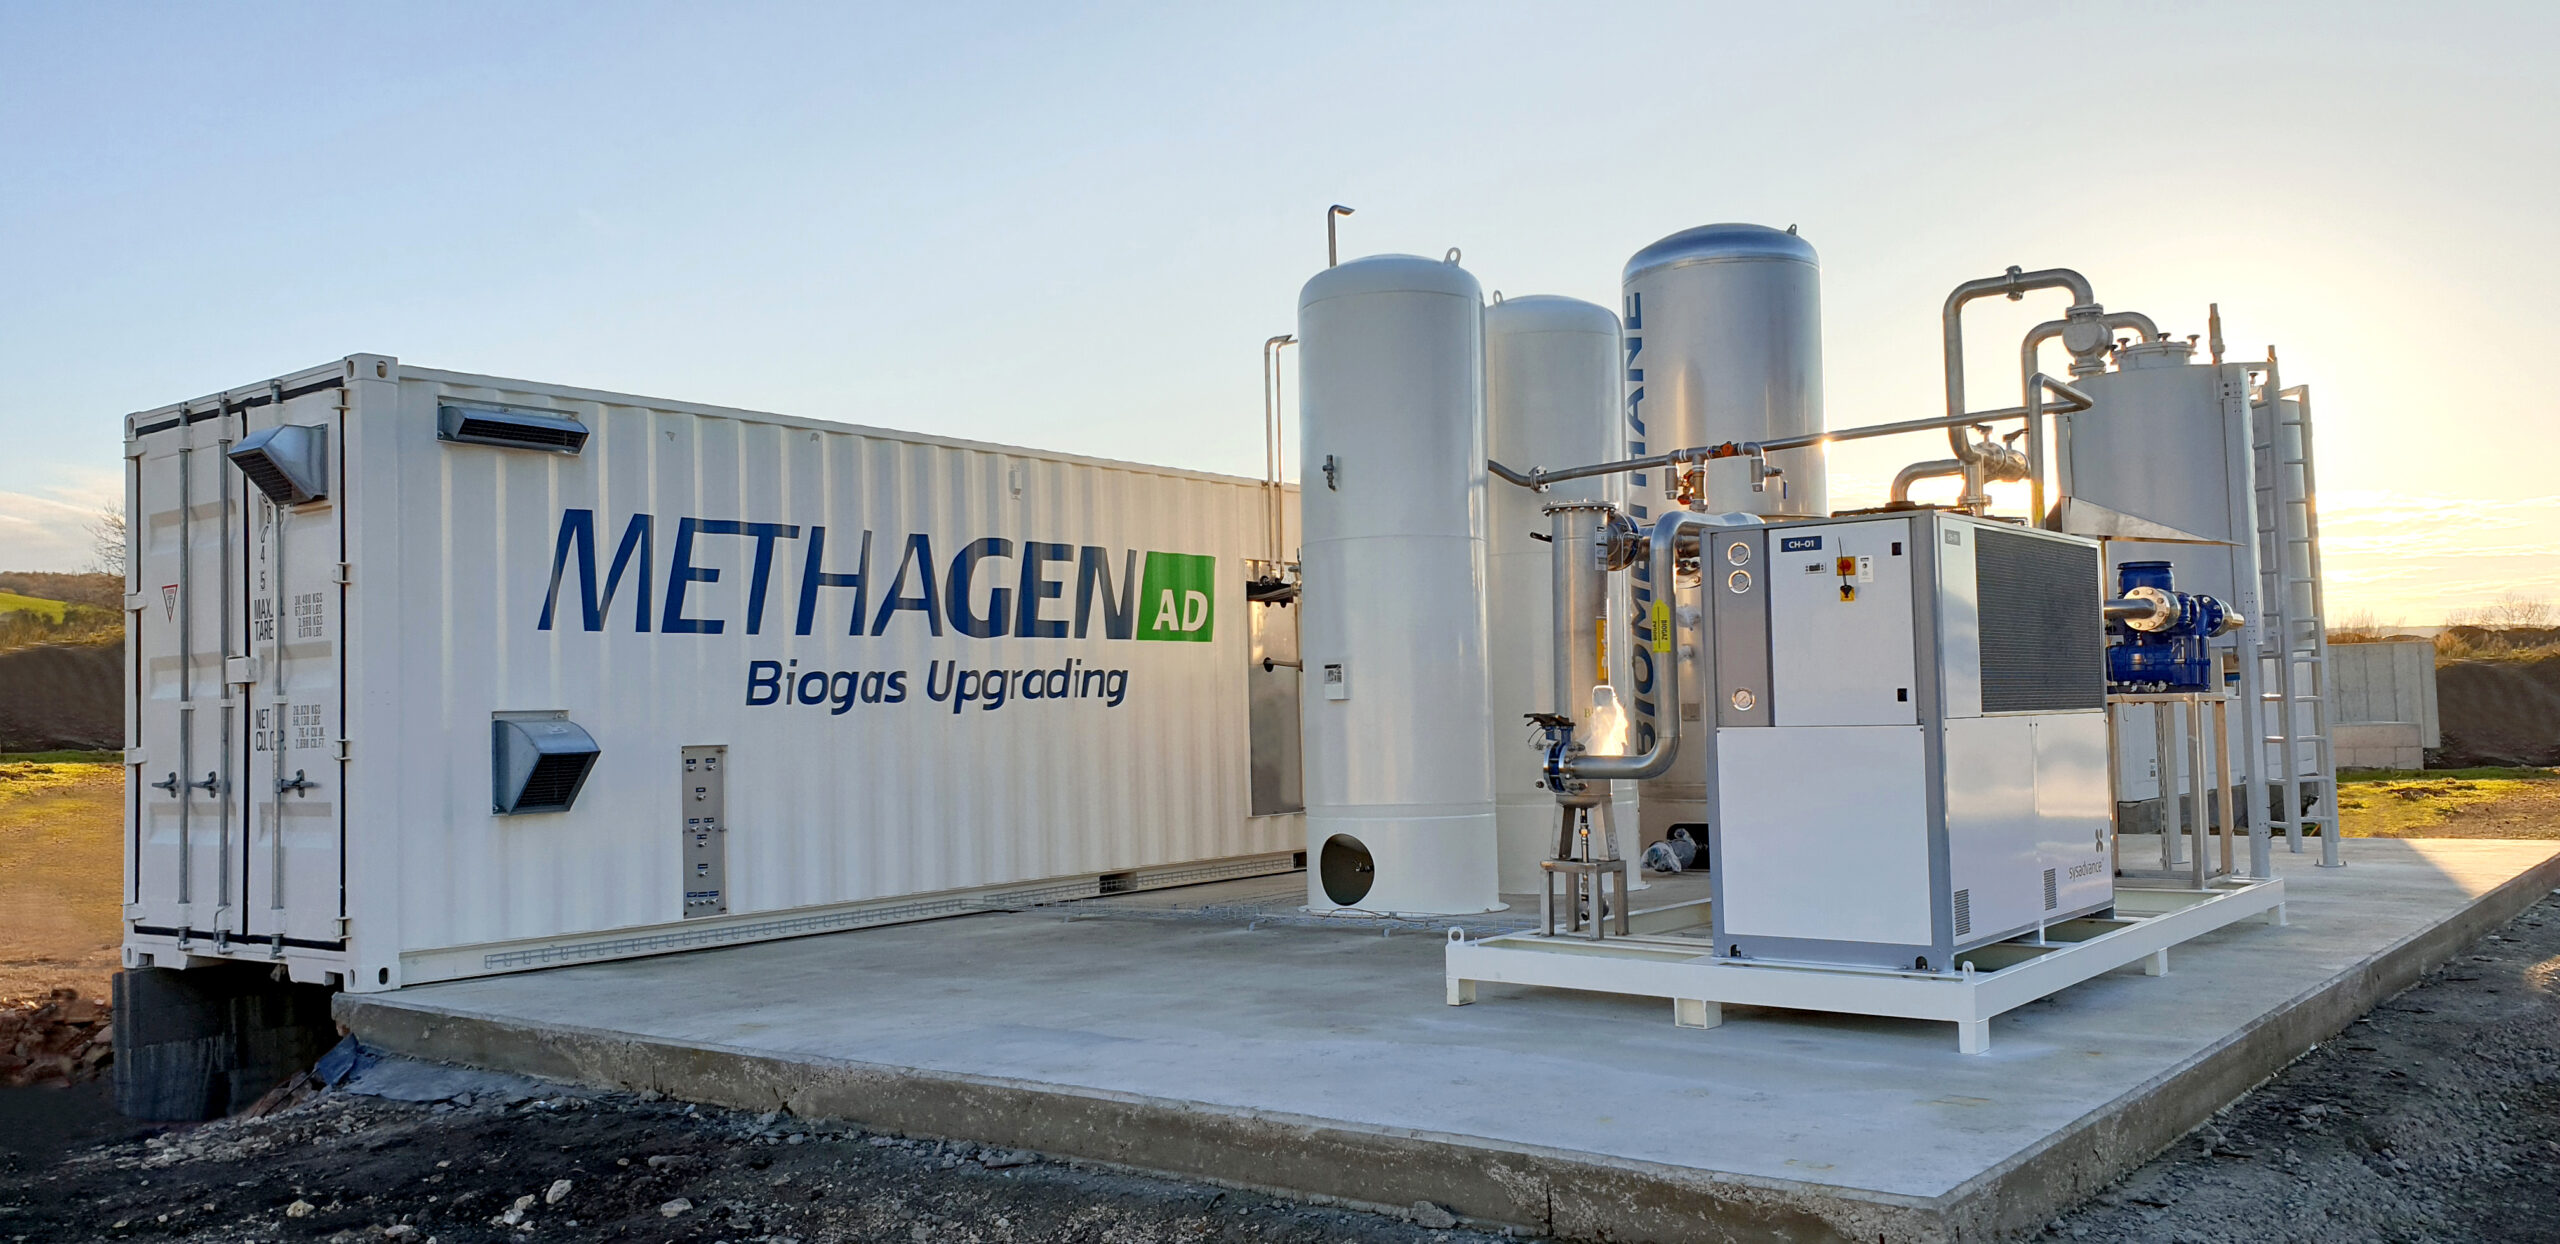
\includegraphics[width=0.85\textwidth]{imgs/metagenad.jpg}
    \caption{Industrial VPSA biomethane upgrading plant. Adapted from Sysadvance}
    \label{fig:metagenad}
\end{figure}

\subsection{VPSA Process} \label{sec:vpsa}

VPSA separates gas components by exploiting their different affinities for porous adsorbent materials under varying pressure conditions. As previously explained, raw 
biogas is primarily composed of methane (CH$_4$) and carbon dioxide (CO$_2$), together with smaller amounts of water vapour and other 
contaminants. Before entering the adsorption unit, the biogas must first be dried to remove the water vapour. This step is essential because the adsorbent 
materials used inside the adsorption columns, one of which is ceramic-based, exhibit a strong affinity for water. Since the adsorption process is exothermic, 
excessive moisture can lead to overheating and permanent damage to the adsorbent material.

After the drying stage, the biogas is compressed before entering the adsorption columns. Operating at elevated pressures increases the probability of gas molecules 
interacting with the adsorbent material, improving the separation efficiency. Each adsorption column is filled with adsorbent materials specifically selected to 
preferentially retain carbon dioxide while allowing methane to pass through. As a result, a methane-rich stream leaves the column and is collected as biomethane.

As the adsorption process continues, the adsorbent gradually becomes saturated with carbon dioxide and loses its separation capacity. At this point, the column 
must be regenerated before it can be reused. Instead of stopping the production process, VPSA systems employ multiple adsorption columns operating simultaneously 
at different stages of the cycle. In the plant considered in this work, four adsorption columns operate in a synchronized sequence, ensuring continuous biomethane 
production while one or more columns undergo regeneration.

Figure~\ref{fig:vpsa} illustrates the operating principle of the four-column VPSA process. During the adsorption stage, compressed biogas enters one of the 
columns, where carbon dioxide is selectively adsorbed while methane exits as the product gas. Once the adsorbent approaches saturation, the column undergoes a 
pressure equalization stage, in which part of the compressed gas is transferred to another column operating at a lower pressure. This step recovers part of the 
compression energy and improves the overall efficiency of the process.

\begin{figure}[htbp]
    \centering
    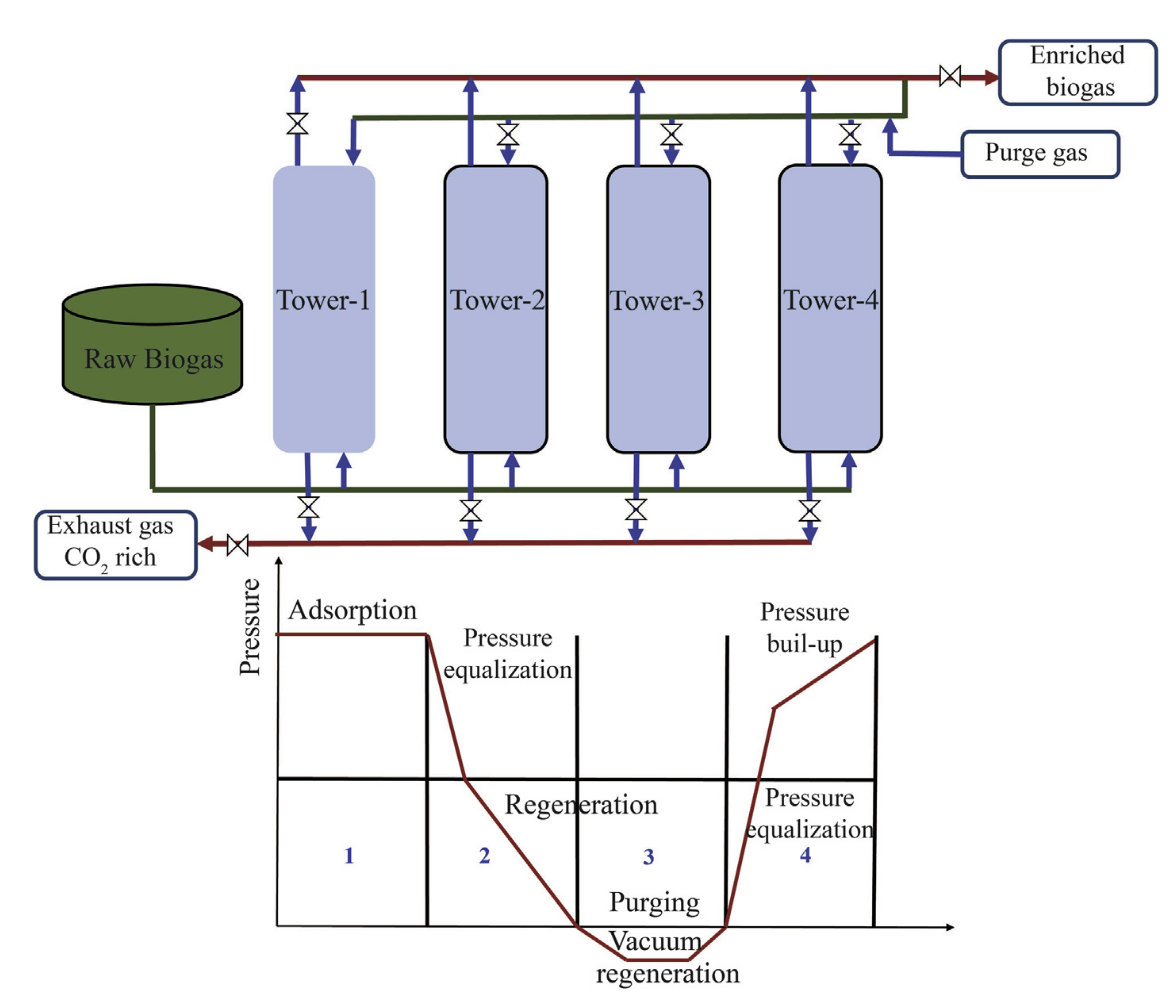
\includegraphics[width=0.70\textwidth]{imgs/vpsa.png}
    \caption{Operating cycle of a four-column VPSA system. Source: \cite{Shah2021}}
    \label{fig:vpsa}
\end{figure}

The column is then depressurized and enters the regeneration stage. Unlike conventional PSA systems, VPSA technology employs a vacuum pump to further reduce the 
pressure below atmospheric conditions. The low pressure promotes the desorption of the retained carbon dioxide, regenerating the adsorbent material and restoring 
its adsorption capacity. Since a small amount of methane is also desorbed during the initial seconds of the vacuum stage, this gas is recovered and redirected to 
the biogas inlet to minimize methane losses.

Finally, the regenerated column is gradually repressurized through another pressure equalization step, followed by pressure build-up until the operating pressure 
is reached. The column is then ready to begin a new adsorption cycle. By continuously alternating the operating stage of each column, the VPSA system is able to 
produce biomethane without interrupting the upgrading process.

In practice, only one adsorption column is in the production stage at any given instant, while the remaining columns are simultaneously undergoing pressure 
equalization, regeneration, or repressurization (\cite{Shah2021}).


\subsection{Vacuum Pump} \label{sec:vacuum}

As discussed in the previous section, the vacuum pump plays a fundamental role in the VPSA process by enabling the regeneration of the adsorption columns. By 
reducing the column pressure below atmospheric conditions, the vacuum pump promotes the desorption of the retained gases, restoring the adsorption capacity of the 
adsorbent material and allowing the adsorption cycle to continue. Consequently, the performance of the vacuum pump has a direct impact on the efficiency, 
productivity, and methane recovery of the entire biomethane upgrading process.

Due to its critical role in the plant operation, the vacuum pump is extensively monitored in the considered biomethane plant. Several process variables, 
including pressure, temperature, electrical current, power consumption, and rotational speed, are continuously acquired to assess its operating condition and 
detect potential abnormal behaviour.

Since this dissertation focuses on the development of AI-based models for AD, FD, and PdM, the vacuum pump was 
selected as the primary component under analysis. Figure~\ref{fig:vacuumpumplive} shows a photograph of a working vacuum pump inside a biogas upgrading plant.

\begin{figure}[htbp]
    \centering
    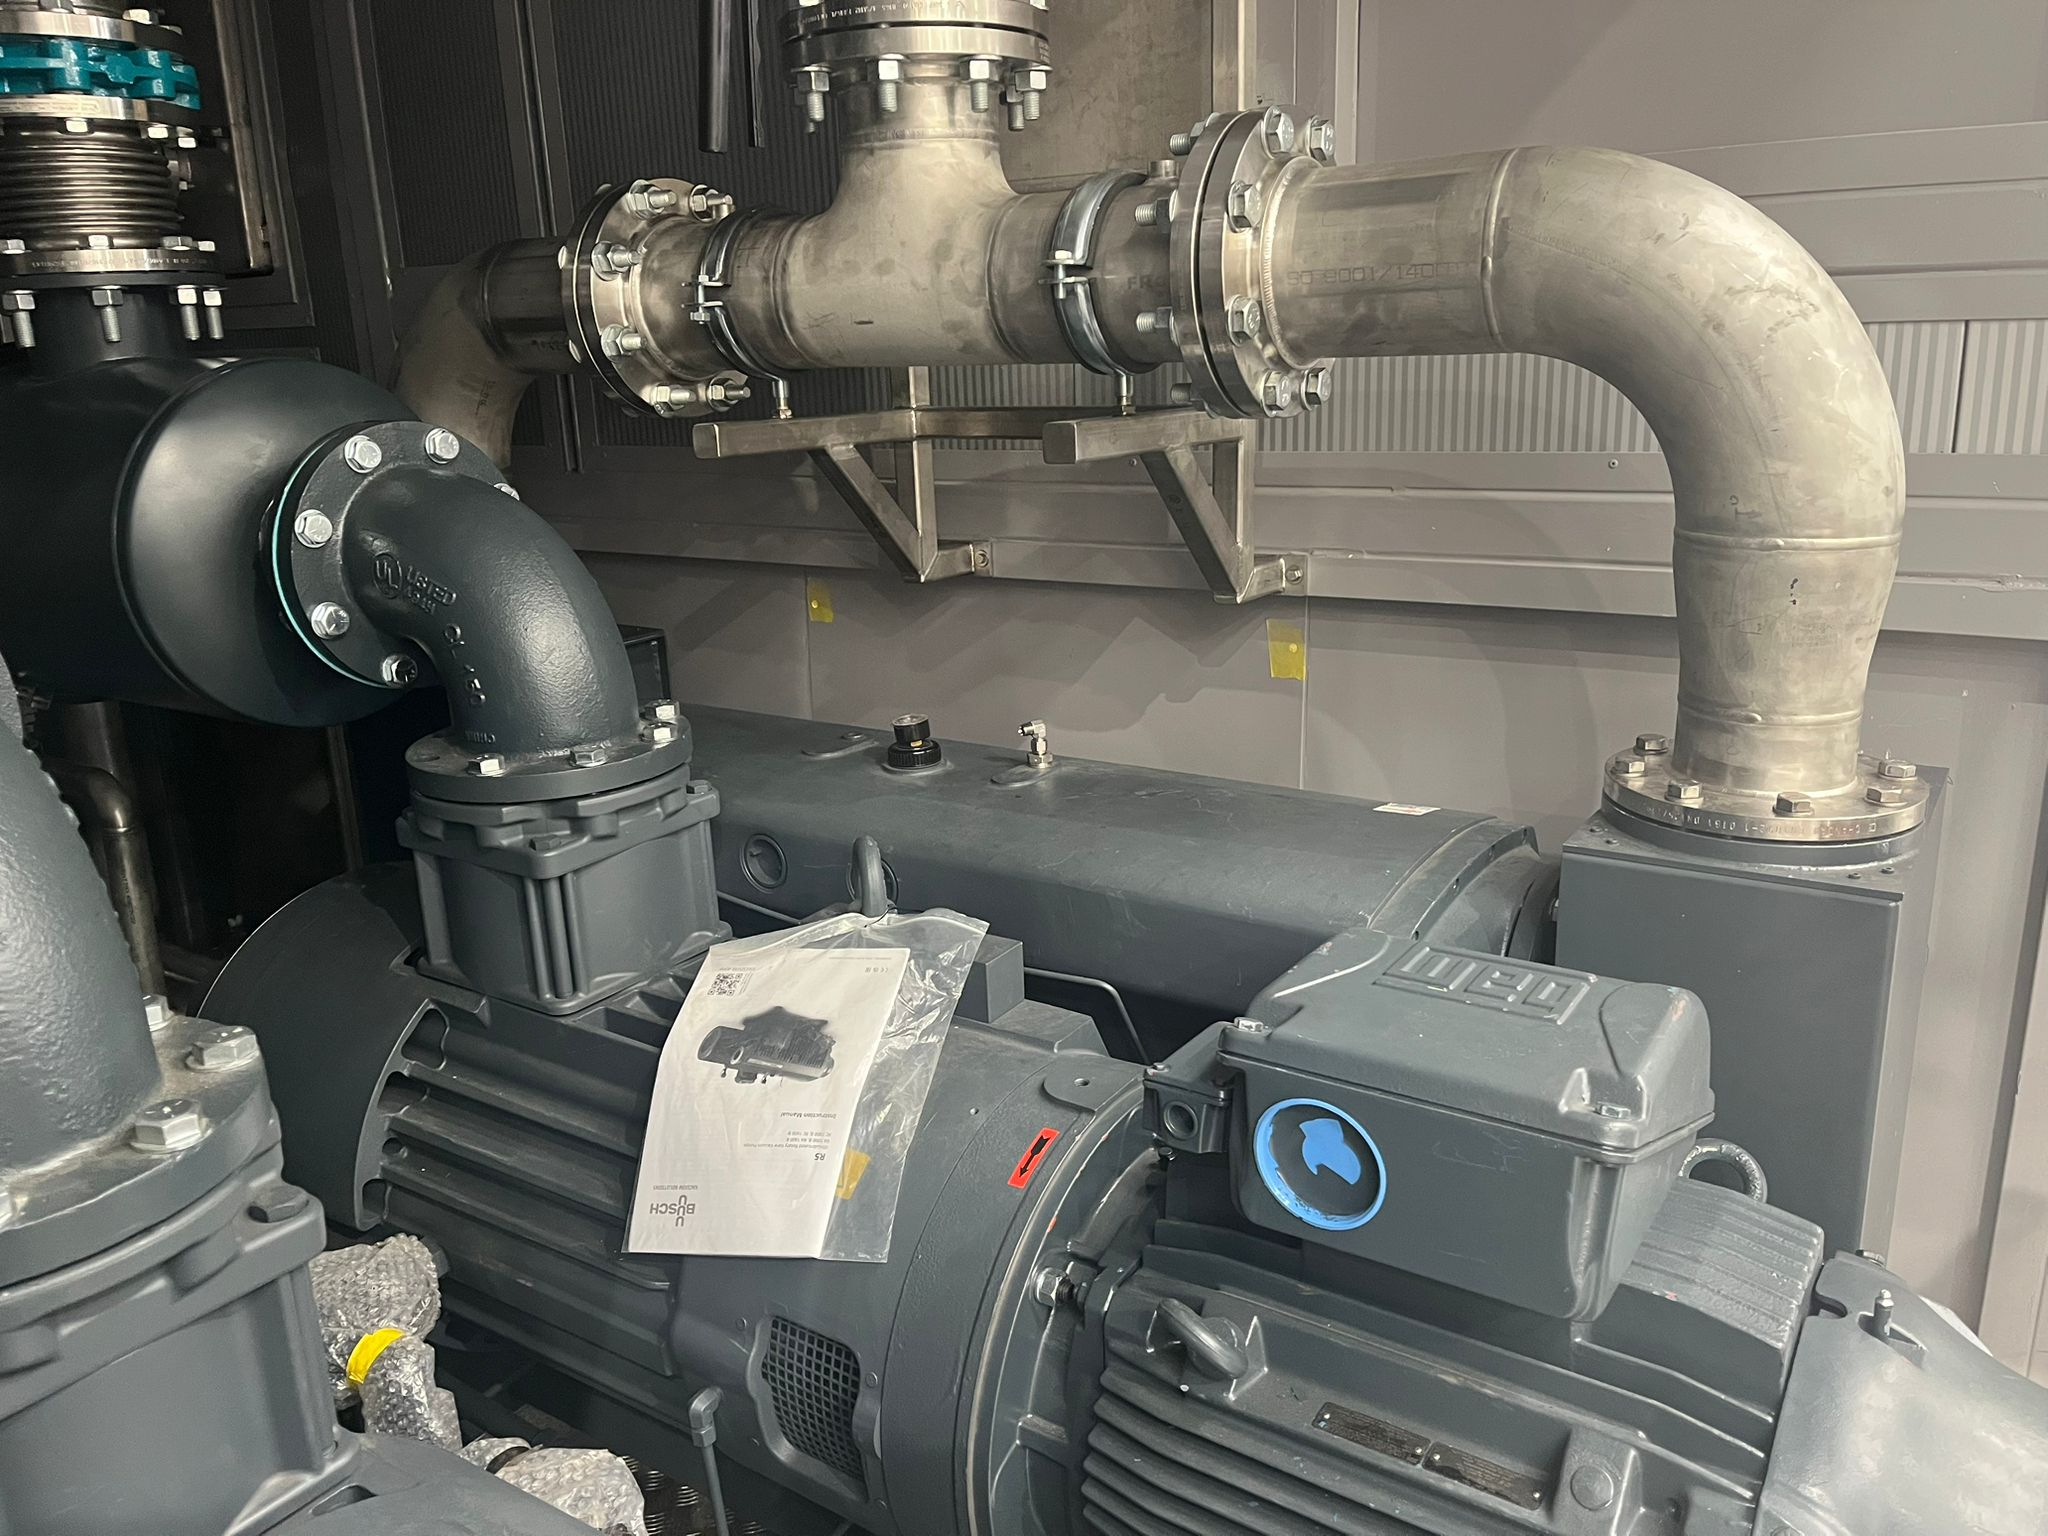
\includegraphics[width=0.50\textwidth]{imgs/vacuum pump.jpeg}
    \caption{Vacuum pump inside a biogas upgrading plant. Adapted from Sysadvance}
    \label{fig:vacuumpumplive}
\end{figure}


\subsubsection{Components} \label{sec:components}

The vacuum pump, whose manufacturer cannot be disclosed due to confidentiality agreements, operates according to the rotary vane principle. Oil plays a 
key role in the pump operation by sealing the clearances between moving parts, providing lubrication, and dissipating the heat generated during gas compression. Figure~\ref{fig:vacuumoperation} illustrates the operating principle 
of the pump, showing the gas flow path during the regeneration stage of the VPSA cycle. Gas extracted from the adsorption column first enters the vacuum pump and is subsequently discharged either back to the biogas inlet or to 
the atmosphere, depending on the operating stage.


\begin{figure}[htbp]
    \centering
    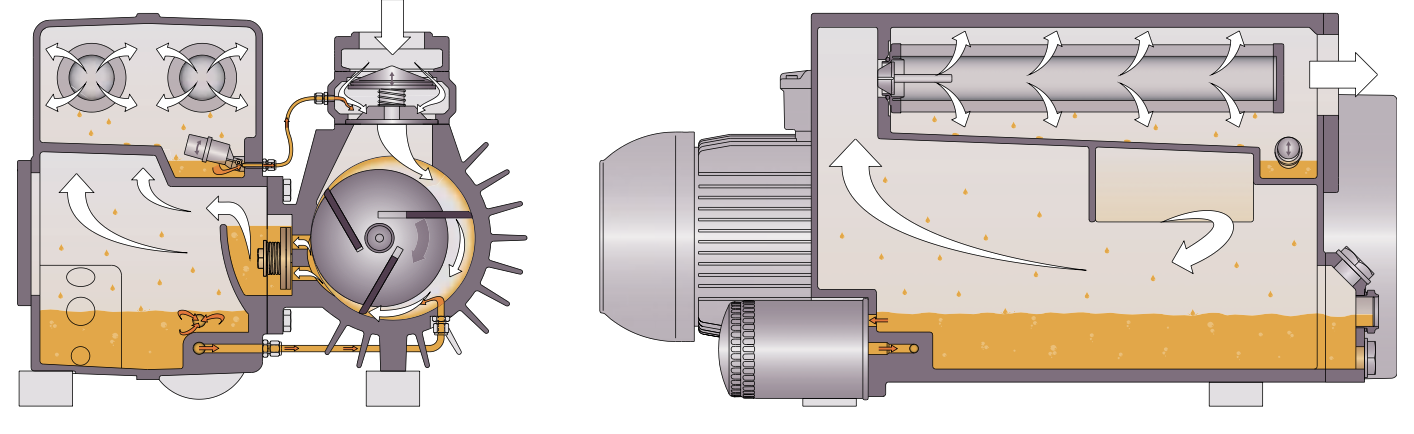
\includegraphics[width=0.80\textwidth]{imgs/vacuumoperation.png}
    \caption{Vacuum pump operating principle. Adapted from the manufacturer's manual}
    \label{fig:vacuumoperation}
\end{figure}

A schematic representation of the pump is also presented in Figure~\ref{fig:vacuumpump}, where the main internal components can be identified. Since a detailed mechanical description of the pump is beyond the scope of this 
dissertation, only the components relevant for understanding the monitored process variables are summarized in Table~\ref{tab:vp_components}.


\begin{figure}[htbp]
    \centering
    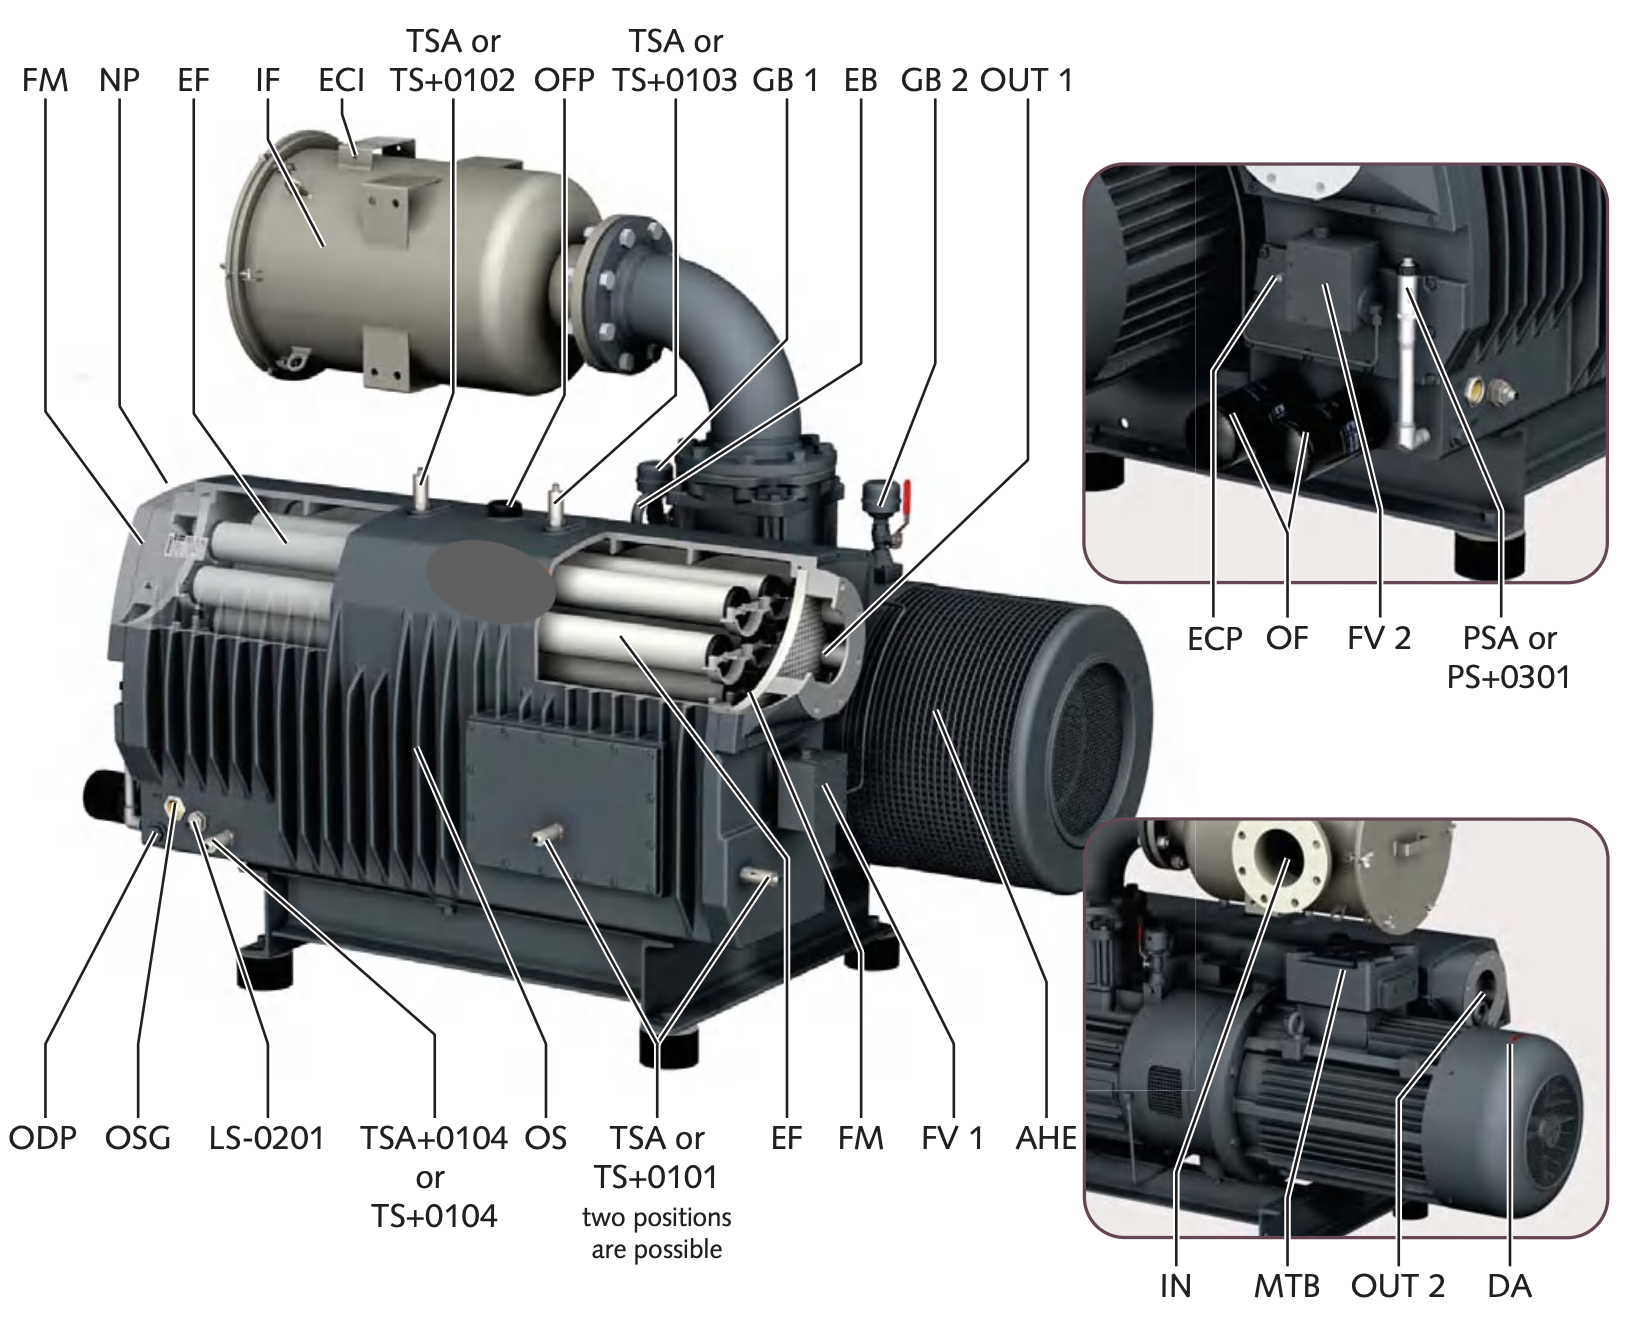
\includegraphics[width=0.79\textwidth]{imgs/vp scheme.png}
    \caption{Vacuum pump scheme. Adapted from the manufacturer's manual}
    \label{fig:vacuumpump}
\end{figure}


\begin{table}[htbp]
\centering
\caption{Main vacuum pump components considered in this dissertation. Adapted from Sysadvance}
\label{tab:vp_components}

\begin{tabular}{ll@{\hspace{1.5cm}}ll}
\hline
\textbf{Abbreviation} & \textbf{Component} &
\textbf{Abbreviation} & \textbf{Component} \\
\hline

TSA &
Resistence Thermometer &
PSA &
Pressure Transmitter \\

TS &
Temperature Switch &
PS &
Pressure Switch \\

LS &
Level Switch &
IF &
Inlet Filter \\

EF &
Exhaust Filter &
OF &
Oil Filter \\

OS &
Oil Separator &
FV &
Float Valve \\

AHE &
Air-Oil Heat Exchanger &
GB &
Gas Ballast Valve \\

\hline
\end{tabular}
\end{table}

\begin{itemize}
    \item \textbf{Gas Ballast Valve (GB):} Introduces a controlled amount of ambient air into the compression chamber to prevent the condensation of vapour inside 
    the pump.
    \item \textbf{Inlet Filter (IF):} Protects the vacuum pump by preventing dust and other solid particles from entering the compression chamber.
    \item \textbf{Exhaust Filter (EF):} Removes oil aerosols from the discharged gas before it is released.
    \item \textbf{Oil Filter (OF):} Removes contaminants from the lubricating oil.
    \item \textbf{Oil Separator (OS):} Separates the lubricating oil from the discharged gas, allowing the recovered oil to be recirculated into the lubrication system.
    \item \textbf{Air-Oil Heat Exchanger (AHE):} Dissipates the heat generated during pump operation by cooling the lubricating oil.
    \item \textbf{Float Valve (FV):} Regulates the oil return from the oil separator to the compression chamber while preventing gas from flowing backwards through 
    the lubrication circuit.
    \item \textbf{Resistance Thermometer (TSA):} Continuously measures the temperature of the gas or lubricating oil, providing analog temperature measurements for 
    process monitoring.
    \item \textbf{Temperature Switch (TS):} Monitors the gas and oil temperatures and generates warning or trip signals when predefined temperature thresholds are exceeded.
    \item \textbf{Pressure Transmitter (PSA):} Continuously measures the pressure inside the oil separator, providing analog pressure measurements used for process monitoring.
    \item \textbf{Pressure Switch (PS):} Monitors the pressure inside the oil separator and activates warning or trip signals when predefined pressure limits are reached.
    \item \textbf{Level Switch (LS):} Monitors the lubricating oil level inside the oil reservoir.
\end{itemize}

\subsubsection{Instrumentation} \label{sec:instrumentation}

To ensure safe and reliable operation, the vacuum pump is equipped with several internal sensors that continuously monitor its operating conditions. 
These sensors measure key process variables, such as pressure, temperature, and oil level, providing real-time information about the pump's health.

In addition to continuous measurements, most sensors are associated with configurable \emph{warning} and \emph{trip} thresholds. A warning signal indicates that a 
monitored variable is approaching an abnormal operating condition. A trip signal corresponds to a critical threshold at which the pump is automatically stopped to 
prevent equipment damage or unsafe operation.

Table~\ref{tab:instrumentation} summarizes the monitored variables together with their corresponding sensors and the associated warning and trip thresholds.

\begin{table}[htbp]
\centering
\caption{Vacuum pump instrumentation and associated protection thresholds. Adapted from the manufacturer's manual.}
\label{tab:instrumentation}

\begin{tabular}{l l c c}
\hline
\textbf{Sensor} & \textbf{Measured Variable} & \textbf{Warning} & \textbf{Trip} \\
\hline
PSA/PS 0301  & Oil separator pressure    & 0.4 bar       & 0.5 bar \\
TSA/0101     & Gas temperature           & 135 $^\circ$C & 140 $^\circ$C \\
TSA/0102     & Gas Temperature           & 105 $^\circ$C & 110 $^\circ$C \\
TSA/0103     & Gas Temperature           & 105 $^\circ$C & 110 $^\circ$C \\
TSA/0104     & Oil temperature           & 90 $^\circ$C  & 110 $^\circ$C \\
\hline
\end{tabular}
\end{table}

In addition to the instrumentation presented above, the vacuum pump also provides the following monitored variables, which are not associated with configurable warning or trip thresholds:

\begin{itemize}
    \item \textbf{Oil Level Sensor:} Monitors the lubricating oil level inside the pump. Only reports whether the oil level is sufficient or low.
    \item \textbf{Pump Current Sensor:} Measures the electrical current drawn by the pump motor, expressed in amperes (A).
    \item \textbf{Pump Power Sensor:} Measures the electrical power consumed by the pump motor, expressed in watts (W).
    \item \textbf{Pump RPM Sensor:} Measures the rotational speed of the pump shaft, expressed in revolutions per minute (RPM).
    \item \textbf{Pump Speed Sensor:} Measures the operating speed of the pump as a percentage of its nominal speed.
\end{itemize}

\subsubsection{Maintenance \& Troubleshooting} \label{sec:maintenance}

Understanding the recommended maintenance procedures and the most common failure possibilities of the vacuum pump is essential for this dissertation. Besides ensuring 
reliable operation of the equipment, this information provides the basis for the fault scenarios considered throughout this work.

According to the manufacturer's manual, preventive maintenance should be performed at regular operating intervals to ensure the reliability and service 
life of the machine. Table~\ref{tab:maintenance} summarizes the recommended maintenance schedule for the main components.

\begin{table}[htbp]
\centering
\caption{Recommended preventive maintenance schedule for the vacuum pump. Adapted from the manufacturer's manual.}
\label{tab:maintenance}

\begin{tabular}{ll}
\hline
\textbf{Task} & \textbf{Maintenance Interval} \\
\hline
Inspect oil level & Daily \\
Check machine for oil leaks & Monthly \\
Check the inlet filter cartridge. Change it if necessary & Monthly \\
Clean the machine from dust and dirt & Every 6 months \\
Clean the Gas Ballast Valve & Every 6 months \\
Check and/or clean the Air-Heat Exchanger & Every 6 months \\
Change the oil, oil filter and the exhaust filter  & Max every 4000 hours, at the latest after 1 year\\
\hline
\end{tabular}
\end{table}

In addition to the recommended maintenance procedures, the manufacturer provides a troubleshooting guide describing the most common faults, their possible causes, 
and the corresponding corrective actions. This information is presented in the following Table~\ref{tab:troubleshooting}.

\begin{table}[htbp]
\centering
\small
\renewcommand{\arraystretch}{1.25}
\caption{Common troubleshooting procedures for the vacuum pump. Adapted from the manufacturer's manual.}
\label{tab:troubleshooting}

\begin{tabularx}{\textwidth}{|p{0.28\textwidth}|X|X|}
\hline
\textbf{Problem} &
\textbf{Possible Cause} &
\textbf{Remedy} \\
\hline

\multirow{3}{*}{The machine does not start.}
&
The motor is not supplied with the correct voltage.
&
Check the power supply. \\
\cline{2-3}
&
The motor is defective.
&
Replace the motor. \\
\cline{2-3}
&
The coupling (CPL) is defective.
&
Replace the coupling (CPL). \\
\hline

\multirow{3}{*}{%
\parbox{0.26\textwidth}{%
The machine does not reach the specified vacuum level.}}
&
Oil level too low.
&
Top up the oil. \\
\cline{2-3}
&
The inlet screen (IS) is partially clogged.
&
Clean the inlet screen (IS). \\
\cline{2-3}
&
The inlet filter cartridge is partially clogged.
&
Replace the inlet filter cartridge. \\
\hline

\multirow{3}{*}{The machine runs very noisily.}
&
Worn coupling (CPL).
&
Replace the coupling (CPL). \\
\cline{2-3}
&
Stuck vanes.
&
Contact the manufacturer for repair. \\
\cline{2-3}
&
Defective bearings.
&
Contact the manufacturer for repair. \\
\hline

\multirow{4}{*}{The machine overheats.}
&
Insufficient cooling.
&
Remove dust and dirt from the machine.\newline
Check the cooling fan. \\
\cline{2-3}
&
Ambient temperature too high.
&
Observe the permitted ambient temperature. \\
\cline{2-3}
&
Oil level too low.
&
Top up the oil. \\
\cline{2-3}
&
The exhaust filters (EF) are partially clogged.
&
Replace the exhaust filters (EF). \\
\hline

\multirow{3}{*}{%
\parbox{0.26\textwidth}{%
The machine fumes or expels oil droplets through the gas discharge.}}

&
The exhaust filters (EF) are partially clogged.
&
Replace the exhaust filters (EF). \\
\cline{2-3}
&
An exhaust filter (EF) O-ring is not fitted properly.
&
Ensure the correct position of the exhaust filters (EF) and the O-rings. \\
\cline{2-3}
&
The float valve (FV) does not operate properly.
&
Check the float valve and the oil return line. Contact the manufacturer if necessary. \\
\hline

\end{tabularx}
\end{table}

Among the various faults identified by the manufacturer, a subset was selected for fault injection in a experimental dataset. These faults were chosen because 
they represent common operating problems that can be reproduced by modifying the monitored process variables while remaining consistent with the physical behaviour 
of the vacuum pump.